
\documentclass[xcolor=dvipsnames]{beamer} 
\usetheme{default} 

\usecolortheme[named=Blue]{structure}
\usetheme[height=7mm]{Rochester} 
\setbeamertemplate{items}[ball] 
\setbeamertemplate{blocks}[rounded]
\setbeamertemplate{navigation symbols}{} 

\usepackage{tikz} 
\usetikzlibrary{shapes.arrows,chains,positioning}

\begin{document}

% -------------------------------------------------------------------------
%
% -------------------------------------------------------------------------

\title{Embedded Languages for Data-Parallel Programming} 
\author[J. Svensson]{Bo Joel Svensson} 
\institute{ 
  Department of Computer Science and Engineering \\ 
  Chalmers University of Technology 
} 

% -------------------------------------------------------------------------
%
% -------------------------------------------------------------------------

\begin{frame}[plain] 
  \titlepage
\end{frame} 


\section{background} 

% -------------------------------------------------------------------------
% What is data parallelism ?
%   * Fine grained
%   * Scalable (more data -> more potential for parallelism) 
%   
% -------------------------------------------------------------------------
\begin{frame}{Data-Parallelism}
\begin{center} 
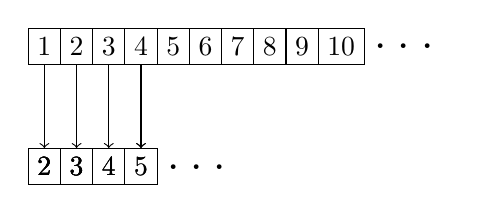
\begin{tikzpicture}[
      start chain=1 going right,start chain=2 going below,node distance=-0.15mm
    ]


  \foreach \x in {1,2,...,10} {
    \node (\x) [draw, on chain=1] {\x};
  }
  \node [on chain=1] {\huge \ldots};
  
  

  \onslide<2>{
    \node [draw, below=3em of 1] (r1) {2};
    \draw [->] (1) -- (r1);
    }

  \onslide<3>{
    \node [draw, below=3em of 1] (r1) {2};
    \node [draw, below=3em of 2] (r2) {3};
    \draw [->] (2) -- (r2);
    }


  \onslide<4>{
    \node [draw, below=3em of 1] (r1) {2};
    \node [draw, below=3em of 2] (r2) {3};
    \node [draw, below=3em of 3] (r3) {4};
    \draw [->] (3) -- (r3);
    }

  \onslide<5>{
    \node [draw, below=3em of 1] (r1) {2};
    \node [draw, below=3em of 2] (r2) {3};
    \node [draw, below=3em of 3] (r3) {4};
    \node [draw, below=3em of 4] (r4) {5};
    \draw [->] (4) -- (r4);
    }
  
  \onslide<6>{
    \node [draw, below=3em of 1] (r1) {2};
    \node [draw, below=3em of 2] (r2) {3};
    \node [draw, below=3em of 3] (r3) {4};
    \node [draw, below=3em of 4] (r4) {5};
    \draw [->] (4) -- (r4);
    \node [right=-0.15mm of r4] {\huge \ldots};
    }
  
\end{tikzpicture} 
\end{center}
\end{frame}

% -------------------------------------------------------------------------
%
% -------------------------------------------------------------------------
\begin{frame}{Data-Parallelism}
\begin{center} 
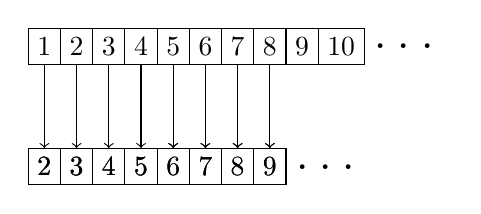
\begin{tikzpicture}[
      start chain=1 going right,start chain=2 going below,node distance=-0.15mm
    ]


  \foreach \x in {1,2,...,10} {
    \node (\x) [draw, on chain=1] {\x};
  }
  \node [on chain=1] {\huge \ldots};
  
  

  \onslide<2>{
    \node [draw, below=3em of 1] (r1) {2};
    \node [draw, below=3em of 2] (r2) {3};
    \node [draw, below=3em of 3] (r3) {4};
    \node [draw, below=3em of 4] (r4) {5};

    \draw [->] (1) -- (r1);
    \draw [->] (2) -- (r2);
    \draw [->] (3) -- (r3);
    \draw [->] (4) -- (r4);
    }

  \onslide<3>{
    \node [draw, below=3em of 1] (r1) {2};
    \node [draw, below=3em of 2] (r2) {3};
    \node [draw, below=3em of 3] (r3) {4};
    \node [draw, below=3em of 4] (r4) {5};
    \node [draw, below=3em of 5] (r5) {6};
    \node [draw, below=3em of 6] (r6) {7};
    \node [draw, below=3em of 7] (r7) {8};
    \node [draw, below=3em of 8] (r8) {9};

    \draw [->] (5) -- (r5);
    \draw [->] (6) -- (r6);
    \draw [->] (7) -- (r7);
    \draw [->] (8) -- (r8);
    }

  \onslide<3>{
    \node [draw, below=3em of 1] (r1) {2};
    \node [draw, below=3em of 2] (r2) {3};
    \node [draw, below=3em of 3] (r3) {4};
    \node [draw, below=3em of 4] (r4) {5};
    \node [draw, below=3em of 5] (r5) {6};
    \node [draw, below=3em of 6] (r6) {7};
    \node [draw, below=3em of 7] (r7) {8};
    \node [draw, below=3em of 8] (r8) {9};

    \draw [->] (5) -- (r5);
    \draw [->] (6) -- (r6);
    \draw [->] (7) -- (r7);
    \draw [->] (8) -- (r8);
    \node [right=-0.15mm of r8] {\huge \ldots};
    }

\end{tikzpicture} 
\end{center}
\end{frame}

% -------------------------------------------------------------------------
% Computing a sum
% -------------------------------------------------------------------------
\begin{frame}{Data-Parallelism}
\begin{center} 
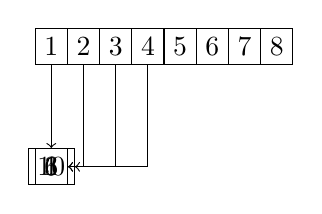
\begin{tikzpicture}[
      start chain=1 going right,start chain=2 going below, node distance=-0.15mm
    ]


  \foreach \x in {1,2,...,8} {
    \node (\x) [draw, on chain=1] {\x};
  }
  % \node [on chain=1] {\huge \ldots};
  
  \onslide<2>{
    \node [draw, below=3em of 1] (r1) {1};
    \draw [->] (1) -- (r1);
    }
  
  \onslide<3>{
    \node [draw, below=3em of 1] (r1) {3};
    \draw [->] (2.south) |- (r1.east);
    }
  
  \onslide<4>{
    \node [draw, below=3em of 1] (r1) {6};
    \draw [->] (3.south) |- (r1.east);
    }

  \onslide<5>{
    \node [draw, below=3em of 1] (r1) {10};
    \draw [->] (4.south) |- (r1.east);
    }




\end{tikzpicture} 
\end{center}
\end{frame}

% -------------------------------------------------------------------------
% Computing a sum in parallel 
% -------------------------------------------------------------------------

\begin{frame}{Data-Parallelism}
\begin{center} 
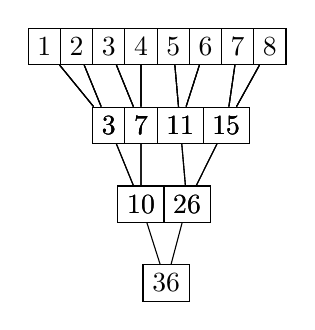
\begin{tikzpicture}[
      start chain=1 going right,start chain=2 going below,node distance=-0.15mm
    ]


  \foreach \x in {1,2,...,8} {
    \node (\x) [draw, on chain=1] {\x};
  }
  %\node [on chain=1] {\huge \ldots};
  
  \onslide<2>{
    \node (imm1) [draw,below=1.5em of 3] {3};
    \node (imm2) [draw,right= of imm1] {7};
    \node (imm3) [draw,right= of imm2] {11};
    \node (imm4) [draw,right= of imm3] {15};
    \draw [-] (1) -- (imm1) 
               (2) -- (imm1)
               (3) -- (imm2) 
               (4) -- (imm2) 
               (5) -- (imm3) 
               (6) -- (imm3) 
               (7) -- (imm4) 
               (8) -- (imm4);
 
  }

  \onslide<3>{
    \node (imm1) [draw,below=1.5em of 3] {3};
    \node (imm2) [draw,right= of imm1] {7};
    \node (imm3) [draw,right= of imm2] {11};
    \node (imm4) [draw,right= of imm3] {15};
    \draw [-] (1) -- (imm1) 
               (2) -- (imm1)
               (3) -- (imm2) 
               (4) -- (imm2) 
               (5) -- (imm3) 
               (6) -- (imm3) 
               (7) -- (imm4) 
               (8) -- (imm4);

    \node (jmm1) [draw,below=1.5em of imm2] {10};
    \node (jmm2) [draw,right= of jmm1] {26};
    
    \draw [-] (imm1) -- (jmm1) 
               (imm2) -- (jmm1) 
               (imm3) -- (jmm2) 
               (imm4) -- (jmm2); 
 
  }

 \onslide<4>{
    \node (imm1) [draw,below=1.5em of 3] {3};
    \node (imm2) [draw,right= of imm1] {7};
    \node (imm3) [draw,right= of imm2] {11};
    \node (imm4) [draw,right= of imm3] {15};
    \draw [-] (1) -- (imm1) 
               (2) -- (imm1)
               (3) -- (imm2) 
               (4) -- (imm2) 
               (5) -- (imm3) 
               (6) -- (imm3) 
               (7) -- (imm4) 
               (8) -- (imm4);

    \node (jmm1) [draw,below=1.5em of imm2] {10};
    \node (jmm2) [draw,right= of jmm1] {26};
    
    \draw [-] (imm1) -- (jmm1) 
               (imm2) -- (jmm1) 
               (imm3) -- (jmm2) 
               (imm4) -- (jmm2); 


    \node (lmm1) [draw,below right=1.5em and -0.8em of jmm1] {36};

    \draw [-] (jmm1) -- (lmm1)
               (jmm2) -- (lmm1); 
 
  }

\end{tikzpicture} 
\end{center}
\end{frame}

% -------------------------------------------------------------------------
%
% -------------------------------------------------------------------------

\begin{frame}{Data-Parallelism}

  Slide with pictures of where you find data-parallelism.

\end{frame}


\begin{frame}{Data-Parallelism}

  \begin{itemize} 
    \item Scalable
    \item Fine grained parallelism
    \item *** CONTINUE 
  \end{itemize} 

\end{frame}

% -------------------------------------------------------------------------
%
% -------------------------------------------------------------------------
\section{GPUs and CUDA}


\begin{frame}{What GPUs look like} 

\end{frame} 

% -------------------------------------------------------------------------
%
% -------------------------------------------------------------------------


\begin{frame}{GPU Programming}
\begin{center} 

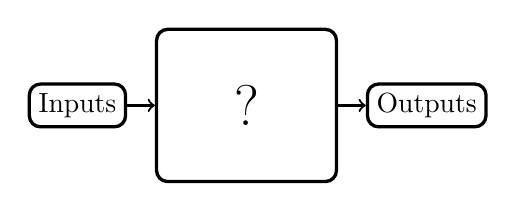
\begin{tikzpicture}[
      start chain=1 going right,start chain=2 going below,node distance=1em,
      every join/.style={->,thick},
    ]

  \node [draw,very thick, rounded corners, on chain=1,join] {Inputs}; 
  \node [draw,very thick, rounded corners, on chain=1,minimum height=5.5em,minimum width = 6.5em,join] {\huge ?}; 
  \node [draw,very thick, rounded corners, on chain=1,join] {Outputs}; 
  

\end{tikzpicture} 
\end{center}

\end{frame}

% -------------------------------------------------------------------------
%
% -------------------------------------------------------------------------
\section{GPUs and CUDA}

\begin{frame}{GPU Programming}
\begin{center} 

\begin{tikzpicture}[remember picture,
      start chain=going right,
      outer/.style={on chain, node distance=1em},
      every join/.style={->,thick},
      inner/.style={circle,draw=blue!50,fill=blue!20,thick,inner sep=1pt},
    ]

  \node [outer,draw,very thick, rounded corners,join] {Inputs}; 
  \node [outer,draw=gray!50,very thick, rounded corners,minimum height=5.5em,minimum width = 6.5em,join] (apa) {
    \begin{tikzpicture} 
      \node [draw=black!100,inner,minimum size=1pt] (k1) {k1};
      \node [draw=black!100,inner,minimum size=1pt, below= 1em of k1] (k2) {k2};
      \node [draw=black!100,inner,minimum size=1pt, right= 1em of k1] (k3) {k3}; 
    \end{tikzpicture}

  }; 
  \node [outer,draw,very thick, rounded corners,join] {Outputs}; 
  

  \draw (k1) -- (k3)
        (k2) -- (k3)
        (apa.west) -- (k1.west)
        (apa.west) -- (k2.west) 
        (k3.east) -- (apa.east); 
  

\end{tikzpicture} 
\end{center}

\end{frame}


% -------------------------------------------------------------------------
%
% -------------------------------------------------------------------------
\section{Embedded Languages}

\begin{frame}{How Bj\"orn and Benny does Embedded Languages} 

\end{frame} 

% -------------------------------------------------------------------------
%
% -------------------------------------------------------------------------
\section{Obsidian}

% -------------------------------------------------------------------------
%
% -------------------------------------------------------------------------
\section{EmbArBB} 

% -------------------------------------------------------------------------
%
% -------------------------------------------------------------------------
\section{Future Work}


\end{document} 
